% ===================================================================
\begin{ex}
	Một người đi xe đạp với tốc độ $v_1=\SI{5}{\meter/\second}$ bên cạnh đường ray tàu hỏa thì thấy một chiếc tàu hỏa chạy qua cùng chiều. Tốc độ của tàu hỏa là $v_2=\SI{15}{\meter/\second}$ đối với mặt đất. Sau thời gian $\SI{15}{\second}$ thì người đó thấy tàu hỏa vượt qua mặt mình. Chiều dài của tàu hỏa là
	\begin{center}
		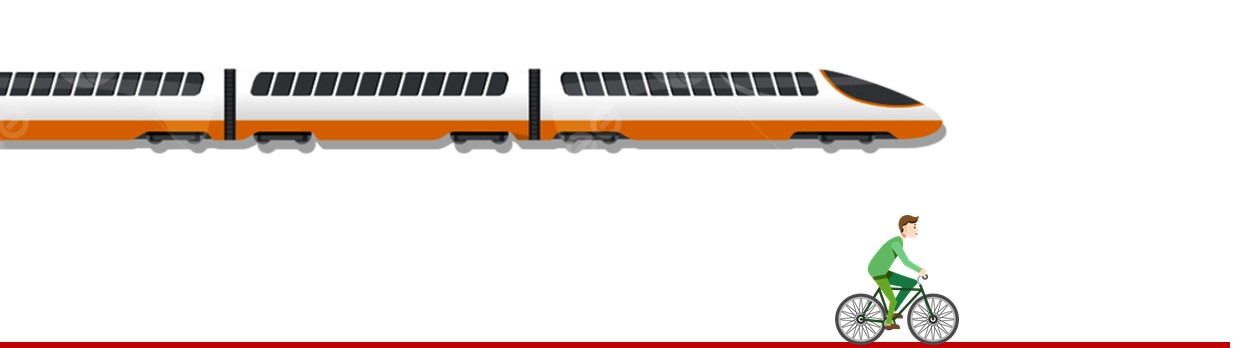
\includegraphics[width=0.4\linewidth]{../figs/D10-1-2}
	\end{center}
	\choice
	{\True $\SI{150}{\meter}$}
	{$\SI{50}{\meter}$}
	{$\SI{100}{\meter}$}
	{$\SI{75}{\meter}$}
	\loigiai{
		Vận tốc tương đối của tàu hỏa so với người:
		$$v_{21}=v_2-v_1=\SI{10}{\meter/\second}$$
		Chiều dài của tàu hỏa:
		$$L=v_{21}t=\SI{150}{\meter}.$$
	}
\end{ex}

% ===================================================================
\begin{ex}
	Một con bọ rùa bò đều trên các cạnh của một tấm ván hình chữ nhật với chiều dài các cạnh $\mathrm{AB}=\SI{40}{\centi\meter}$, $\mathrm{BC}=\SI{20}{\centi\meter}$, mỗi 2 giây nó bò được $\SI{1.5}{\centi\meter}$. Tại thời điểm ban đầu, con bọ rùa ở đỉnh A của tấm ván. Kể từ thời điểm ban đầu, trong thời gian $\SI{80}{\second}$, vận tốc trung bình và tốc độ trung bình của con bọ rùa lần lượt là	
	\choice
	{$\SI{0.75}{\centi\meter/\second}$, $\SI{0.75}{\centi\meter/\second}$}
	{$\SI{0.75}{\centi\meter/\second}$, $\SI{0.56}{\centi\meter/\second}$}
	{\True $\SI{0.56}{\centi\meter/\second}$, $\SI{0.75}{\centi\meter/\second}$}
	{$\SI{0.56}{\centi\meter/\second}$, $\SI{0.56}{\centi\meter/\second}$}
	\loigiai{}
\end{ex}